% Template: Fabian Wenzelmann, 2016 - 2017

\documentclass[a4paper,
  twoside, % für Unterscheidung gerade / ungerade Seite
  headlines=2.1 % Anzahl der Zeilen im Kopf, wenn man mehr verwenden will erhöhen
  ]{scrartcl}
\usepackage[
  margin=2cm,
  includefoot,
  footskip=35pt,
  includeheadfoot,
  headsep=0.5cm,
]{geometry}
\usepackage[ngerman]{babel}
\usepackage{graphicx}
\usepackage[utf8]{inputenc}
\usepackage{caption}
\usepackage{amsmath}
\usepackage{amssymb}
\usepackage[automark,headsepline]{scrlayer-scrpage}
\usepackage{enumerate}
\usepackage[protrusion=true,expansion=true, kerning]{microtype} % Sieht damit einfach schöner aus

\newcommand{\yourname}{Simon Schuler \and Jannik Thoma} % Weitere Autor*innen mittels \and Befehl einfügen
% \newcommand{\yourname}{Dein Name \\ \texttt{123456789} \and Anderer Name \\ \texttt{987654321}} % Hier ein Bsp mit Martikelnummern, auf jeden Fall \headingname anpassen (keine newlines)
\newcommand{\headingname}{\yourname} % Namen wie sie im Kopf erscheinen, wenn zu lang z.B. nur Nachnamen verwenden
% Auch wenn man eine Trennung durch Kommata haben will hier die Namen erneut durch Kommata getrennt wiederholen
% \newcommand{\headingname}{Dein Name, Anderer Name} % Hier ein Beispiel für eine anders formatierte Liste
\newcommand{\lecture}{Mathe 1}
\newcommand{\sheetnum}{4}
\newcommand*{\QED}{\hfill\ensuremath{\square}}%
\author{\yourname}
\title{\lecture}
\subtitle{Übungsblatt \sheetnum}
\date{} % Wer ein Datum auf dem Dokument haben will hier eintragen, \today erstellt das heutige Datum

\pagestyle{scrheadings}
\setkomafont{pagehead}{\normalfont}
\lohead{\lecture\\\headingname}
\lehead{\lecture\\\headingname}
\rohead{Übungsblatt \sheetnum}
\rehead{Übungsblatt \sheetnum}


\begin{document}

\maketitle

% Hier kommt dein eigentlicher LaTeX Code
\section*{Aufgabe 1}
\subsection*{(a)}
\begin{figure}[h!]
\centering
\includegraphics[width=0.7\linewidth]{../../../Bilder/w04_TI}
\caption[Schaltkreis 1]{SK 1}
\label{fig:w04_TI}
\end{figure}

\subsection*{(b)}
Tiefe = 3, Kosten = 5\\
\subsection*{(c)}
\begin{align*}
	v_2 &= (x_1 \land x_2)\lor (x_3\land (x1 \oplus x_2))\\
	v_4 &= (x_3 \oplus (x_1 \oplus x_2))
\end{align*}
    
\section*{Aufgabe 2}
\subsection*{(a)} 
\begin{tabular}{c|c|c|c||c}
	f & w & z & k & e \\
	\hline
		0&0&0&0&0\\
		0&0&0&1&0\\
		0&0&1&0&0\\
		0&0&1&1&1\\
		0&1&0&0&0\\
		0&1&0&1&0\\
		0&1&1&0&1\\
		0&1&1&1&1\\
		1&0&0&0&1\\
		1&0&0&1&1\\
		1&0&1&0&0\\
		1&0&1&1&0\\
		1&1&0&0&1\\
		1&1&0&1&0\\
		1&1&1&0&0\\
		1&1&1&1&0
\end{tabular}
\subsection*{(b/c)}
$	e = \bar{f}\bar{w}zk \lor \bar{f}wz\bar{k}\lor \bar{f}wzk \lor f\bar{w}\bar{z}\bar{k} \lor f \bar{w}\bar{z}k \lor fw\bar{z}\bar{k}$

\subsection*{(d)}

	$\bar{e} = (f\lor w\lor z\lor k) \land (f\lor w \lor z \lor \bar{k}) \land (f \lor w \lor \bar{z} \lor k) \land (f\lor \bar{w}\lor z\lor k) \land (f\lor \bar{w} \lor z\lor \bar{k}) \land (\bar{f}\lor w\lor \bar{z}\lor k) \land (\bar{f}\lor w\lor \bar{z}\lor \bar{k})\land (\bar{f}\lor \bar{w}\lor z \lor \bar{k})\land (\bar{f} \lor \bar{w} \lor \bar{z} \lor k) \land (\bar{f}\lor \bar{w} \lor \bar{z} \lor \bar{k}) $
\subsection*{(e)}
Der Farmer kann es schaffen, indem er alle Zustände der DNF ($e$) aus b/c vermeidet und nur Zustände der KNF($\bar{e}$) abläuft.
\section*{Aufgabe 3}
\subsection*{(a)}
\begin{center}
	\centering
	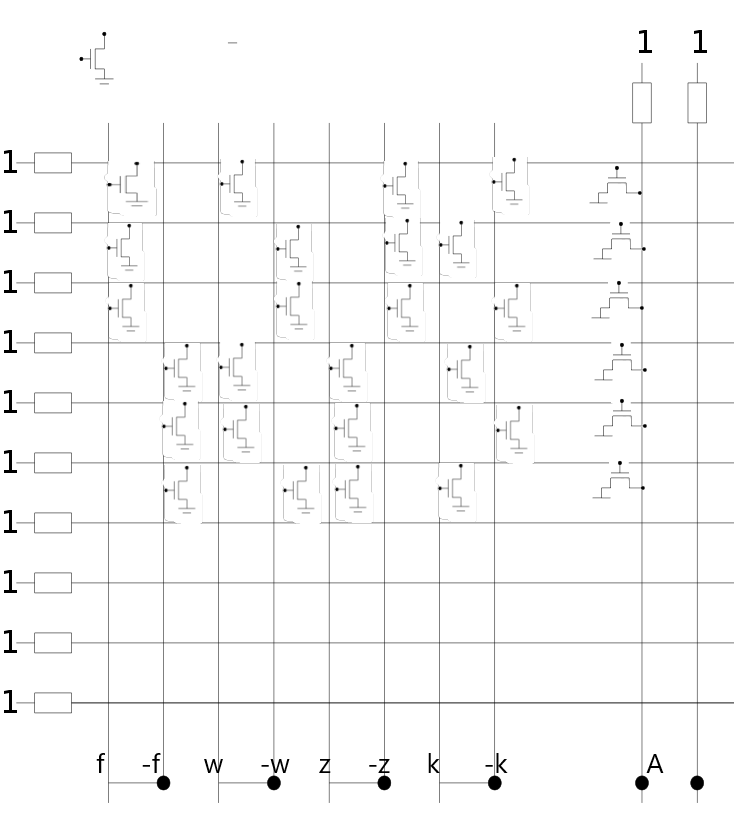
\includegraphics[width=0.8\textwidth]{pla1.png}
	\label{fig:Schaltung}
\end{center}
\subsection*{(b)}
$cost_1(PLA) = 6, \quad cost_2(PLA) = 6\cdot 4 +6 = 30$
\section*{Aufgabe 4}
\subsection*{(a)}
\begin{flalign*}
	f_1 : &\bar{x_1}\bar{x_2}\bar{x_3}x_4 \lor\\
	&x_1 \bar{x_2}\bar{x_3}x_4 \lor\\
	&x_1 \bar{x_2} x_3 \bar{x_4}\lor\\
	&x_1 \bar{x_2}x_3 x_4\lor\\
	&x_1 x_2 \bar{x_3} x_4 \lor\\
	&x_1 x_2 x_3 x_4
\end{flalign*}
\begin{flalign*}
	f_2 : &\bar{x_1}\bar{x_2}x_3 x_4 \lor\\
	&\bar{x_1} x_2 \bar{x_3} \bar{x_4} \lor\\
	&\bar{x_1} x_2 \bar{x_3} x_4 \lor\\
	&\bar{x_1} x_2 x_3 x_4 \lor \\
	&x_1 x_2 \bar{x_3} x_4\lor\\
	&x_1 x_2 x_3 x_4
\end{flalign*}
\subsection*{(b)}
\begin{center}
\centering
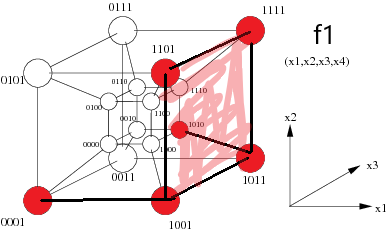
\includegraphics[width=0.7\linewidth]{hypercubef1blatt4}
\label{fig:hypercubef1blatt4}
\end{center}
\begin{center}
\centering
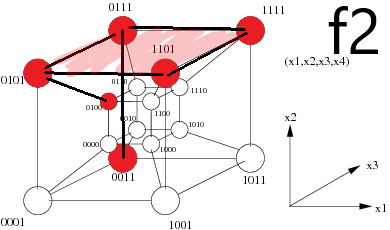
\includegraphics[width=0.7\linewidth]{hypercubef2blatt4}
\label{fig:hypercubef2blatt4}
\end{center}
\subsection*{(c)} 
\begin{align*}
	f_1) \quad g_1 &= \bar{x_2}\bar{x_3}x_4 \lor\\
	&x_1 x_2 \lor\\
	&x_1 \bar{x_2} x_3
\end{align*}
\begin{align*}
	f_2) \quad g_2 &= \bar{x_1} x_3 x_4 \lor \\
	&x_2 x_2 \lor \\
	&\bar{x_1} \bar{x_2} \bar{x_3} 
\end{align*}

\end{document}
